\documentclass[11pt,sigconf]{acmart}

\usepackage{booktabs} % For formal tables

\graphicspath{{figure/}{figures/}}

% Copyright
%\setcopyright{none}
%\setcopyright{acmcopyright}
%\setcopyright{acmlicensed}
\setcopyright{rightsretained}
%\setcopyright{usgov}
%\setcopyright{usgovmixed}
%\setcopyright{cagov}
%\setcopyright{cagovmixed}


% DOI
\acmDOI{10.475/123_4}

% ISBN
\acmISBN{123-4567-24-567/08/06}

%Conference
\acmConference[Spring '22]{CSCI 6502 - Big Data Analytics}{Mar '22}{Boulder , CO, USA} 
\acmYear{2022}
\copyrightyear{2022}

\acmPrice{15.00}


\begin{document}
\title{Galaxy Morphological Classification: An Analysis of Large Spectral and Photometric Datasets}
\titlenote{Produces the permission block, and copyright information}
\subtitle{Extended Abstract}

\author{Son Pham}
\authornote{Note}
\orcid{1234-5678-9012}
\affiliation{%
  \institution{CU Boulder}
  \city{Boulder} 
  \state{CO} 
}
\email{son.pham-2@colorado.edu}


% The default list of authors is too long for headers}
\renewcommand{\shortauthors}{S. Pham}


\begin{abstract}

\end{abstract}

%
% The code below should be generated by the tool at
% http://dl.acm.org/ccs.cfm
% Please copy and paste the code instead of the example below. 
%
\begin{CCSXML}
  <ccs2012>
  <concept>
  <concept_id>10002950.10003714</concept_id>
  <concept_desc>Mathematics of computing~Mathematical analysis</concept_desc>
  <concept_significance>300</concept_significance>
  </concept>
  <concept>
  <concept_id>10002951.10002952</concept_id>
  <concept_desc>Information systems~Data management systems</concept_desc>
  <concept_significance>300</concept_significance>
  </concept>
  <concept>
  <concept_id>10010147.10010257</concept_id>
  <concept_desc>Computing methodologies~Machine learning</concept_desc>
  <concept_significance>300</concept_significance>
  </concept>
  <concept>
  <concept_id>10010147.10010919</concept_id>
  <concept_desc>Computing methodologies~Distributed computing methodologies</concept_desc>
  <concept_significance>300</concept_significance>
  </concept>
  </ccs2012>
\end{CCSXML}

\ccsdesc[300]{Mathematics of computing~Mathematical analysis}
\ccsdesc[300]{Information systems~Data management systems}
\ccsdesc[300]{Computing methodologies~Machine learning}
\ccsdesc[300]{Computing methodologies~Distributed computing methodologies}
\ccsdesc[300]{Applied computing~Astronomy}

% We no longer use \terms command
%\terms{Theory}

\keywords{ACM proceedings}


\maketitle

\section{Introduction}

% Refer to \verb|acmart.pdf| \cite{veytsmanlatex} (\url{https://www.ctan.org/pkg/acmart}, 
% \url{http://www.acm.org/publications/proceedings-template}) for additional examples and instructions.
Big data analytics is transforming the way scientists and astronomers study the universe. 
With each large scale telescope on the ground or in space, dozens of gigabytes of data 
is being generated per day - an amount that will take an increasingly amount of time
to explore and process. For example, the Hubble Space Telescope generates about 120G of 
scientific data every week \cite{tillman}. Sky surveys conducted by telescopes such as
the Sloan Digital Sky Survey (SDSS) produces data releases each year that can be as high as
100's of TBs. SDSS provides a wide range of data types, such as optical spectra,
infrared spectra, and imaging. 
\\
Recent discoveries, such as the presence of over 1000 black holes 
in the center of our Milky Way, was realized using data from decades ago generated by
the Chandra satellite \cite{sagittarius}. Scientific and technological advancement in 
combination led the 
way to this capability. With the increase in computational performance, astronomers 
now have the capabilities to explore these large datasets without the need to invest 
in large ground-based optical telescopes or work in a research lab. 
As big data analytics continue to grow, these discoveries will become more common as 
scientists continue to collect and process more of the data that is available. As technological
advancements grow, they will have more readily available tools and platforms for their 
analysis. With the cummilation telescopes and technologies present today, the entire 
electromagnetic spectrum can be observed within a patch of sky of interest. 
\\
SDSS datasets, such provide many different data types, provides the opportunity to
explore galaxies, stars, and quasars too distant to view for amateur astronomers and 
conduct many different types of analysis on them. The analytics of interest to the
authors include the use of optical imaging and spectral data. Legacy imaging generated 
from prior SDSS programs, if used with machine learning classification techniques, 
can provide automatic classification of morphological properties of these galaxies. 
Quatities measured from these images and spectra readings can also provide information
such as magnitudes, redshifts, and object classifications. In particular, redshift can
be a good indicator of galaxy morphology. 
\\
This paper will go over in detail the approach to perform morphological classification of 
galaxies using these available information from various sources. The main source of interest
for the author is SDSS's data, which includes 100's of terabytes of data covering more
than one-third of the entire celestial sphere \cite{abdurro}.


\section{Literature Survey}

Sky surveys provide a plethora of data for scientists to study and observed. Many different 
studies were conducted with data collected from satellites and telescopes around the world. 
The field of morphological classification, in particular, is rich in the research of techniques 
and methods to analyze these large datasets and help classify galaxies. Galaxy Zoo, a program 
that spearheaded the galaxy morphological classification manually conducted by volunteer 
astronomers around the world \cite{galaxyzoo1} \cite{galaxyzoo2}. 
\\  
G. Martin et al conducted studies on galaxy morphological classification using unsupervised 
machine learning techniques \cite{gmartin}. The technique the authors proposed does not require 
classified data, which is beneficial for new surveys that does not come with class labels. In the 
method proposed, clustering was used to present graphs that represent image patches with 
similar visual properties, which can be used to group similar galaxies together. 
\\
H. Dominguez Sanchez et al. studied machine learning techniques to improve the 
classification process, particularly in the field of deep learning \cite{hsanchez}. 
This process utilized existing visual classification catalogues with neural network models. 
Convolutional Neural Networks were trained using two visual classification catalogues: 
the Galaxy Zoo 2 similar to the current project's were used to train the geometric parameters 
that makes up a galaxy, and the Nair \& Abraham datasets for imaging attributes. 
\\
P. H. Barchi et al. presented a paper on comparing various galaxy morphological classification 
techniques and provided suggestions on how to substantially improve the classification 
process \cite{phbarchi}. 



\section{Datasets}

The main dataset source used in this project is the Sloan Digital Sky Survey (SDSS). 
SDSS provides all the data captured from its instruments and encompasses over one-third
of the entire celestial sphere. The latest data release from SDSS is Data Release 17 in
December 2021 \cite{abdurro}, with an overview shown in Table \ref{tab:table_SDSS}. 

\begin{table}[]
  \begin{tabular}{ |p{4.0cm}|p{2.0cm}|p{1.3cm}|  } \hline
   \textbf{Parameter} & \textbf{Description} & \textbf{Unit}  \\ \hline
   Total unique area covered & 14,555  & sq. deg \\ \hline
   Total area of imaging (including overlaps) & 31,637 & sq. deg \\ \hline
   Individual image field size & 1361x2048 (0.0337) & pixels (sq. deg) \\ \hline
   catalog objects & 1,231,051,050 & (-) \\ \hline
   unique detections & 932,891,133 & (-) \\ \hline
   Median PSF FWHM, r-band & 1.3 & arcsec \\ \hline
   Pixel scale & 0.396 & arcsec \\ \hline
  \end{tabular}
  \caption{\label{tab:table_SDSS}SDSS Dataset Sky Coverage \cite{abdurro}}
\end{table}

The main source used within SDSS was the data collected from their imaging system, 
which contains objects for about one-third of the entire night sky. Five broad 
bands were defined and used by SDSS imaging camera, namely "u-g-r-i-z", which 
are the five rows of Charge Couple Devices (CCD's) used by the imaging camera. 
The central wavelengths of the filters are shown in Table \ref{tab:table_filters}, 
and a plot of the response curves of the color band is shown in 
Figure \ref{fig:colorbands}, which shows the throughput that defines the photometric 
system. More information on the camera system can be found on the SDSS 
imaging website \cite{sdss_imaging}. 

\begin{table}[]
  \begin{tabular}{ |p{2.2cm}|p{2.6cm}|  } \hline
   \textbf{Filter Band} & \textbf{Wavelength (\AA)} \\ \hline
   u & 3551 \\ \hline
   g & 4686 \\ \hline
   r & 6166 \\ \hline
   i & 7480 \\ \hline
   z & 8932 \\ \hline
  \end{tabular}
  \caption{\label{tab:table_filters}SDSS Color-band Filters \cite{sdss_imaging}}
\end{table}

\begin{figure}[htbp]
  \centering
  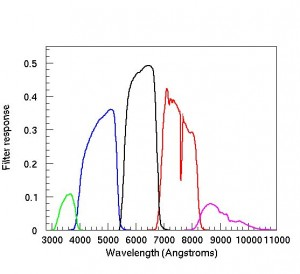
\includegraphics[scale=0.5]{camera_filters-300x274}
  \caption{SDSS Imaging Colorbands \cite{sdss_imaging}}
  \label{fig:colorbands}
\end{figure}

Although the images is not currently being used in the project, data from the five 
color bands are. This dataset contained almost half a billion unique 
objects (stars, galaxies, etc.), with many parameters, though only a selected 
number of key parameters were used in the machine learning model, shown in 
Table \ref{tab:table_IMAGE}. the celestial right ascension and declination is used to 
locate the object in the celestial sphere and to cross-match across other data sources. 
The color bands are used to determine the dominant filter bands present in an object and 
determine redshift. Adaptive 4th moments of object intensity are measured using a radial 
Gaussian weight function, teratively adapted to the shape and size of the object. The 
radius containing the 50\% and 90\% total Petrosian flux in each band is used to 
determine the concentration of light for an object, which is the ratio of the radius 
from the center of an object to the radius containing 50\% and 90\% of the total 
Petrosian flux. Reference \cite{galaxy_photometry} provides an overview of using 
Petrosian flux to determine the shape of a galaxy.

\begin{table}[]
  \begin{tabular}{ |p{3.0cm}|p{3.2cm}|p{1.0cm}|  } \hline
   \textbf{Parameter} & \textbf{Description} & \textbf{Unit}  \\ \hline
   Objid & object id  & - \\ \hline
   ra & Celestial Right Ascension & deg \\ \hline
   dec & Celestial Declination & deg \\ \hline
   u,g,r,i,z & SDSS color-band filters & \AA \\ \hline
   mCr4\_u/g/r/i/z & Adaptive 4th moments of object intensity & (-) \\ \hline
   petroR50\_u/g/r/i/z petroR90\_u/g/r/i/z & Radius containing 50/90\% total Petrosian Flux in each band & arcsec \\ \hline
  \end{tabular}
  \caption{\label{tab:table_IMAGE}SDSS Photometric Parameters Used}
  \end{table}

Another data source used from the SDSS are the optical spectra data collected by the 
Extended Baryon Oscillation Spectroscopic Survey (eBOSS) \cite{galaxy_eboss}. In essense,
the mission of eBOSS is to measure the expansion history of the Universe, focusing on 
observations of galaxies and quasars, in particularly the rate of change of 
distances of these objects (redshift). Table \ref{tab:table_eboss} lists the parameters 
used from this dataset. As better understanding of the survey is obtained, additional 
parameters may be used to increase model fidelity.  

\begin{table}[]
  \begin{tabular}{ |p{1.8cm}|p{4.0cm}|p{1.0cm}|  } \hline
   \textbf{Parameter} & \textbf{Description} & \textbf{Unit}  \\ \hline
   bestobjid & recommended SDSS object match  & - \\ \hline
   class & best spectroscopic match (star, galaxy, qso) & - \\ \hline
   subclass & best spectroscopic subclassification & - \\ \hline
   z & best redshift & \AA \\ \hline
   zerr & error in best redshift & - \\ \hline
  \end{tabular}
  \caption{\label{tab:table_eboss}eBOSS Spectro Parameters Used}
  \end{table}

The final dataset currently used in the project is the morphological classification dataset 
from Galaxy Zoo, which contains classifications for nearly 900,000 galaxies. To better 
understand details about a galaxy that cannot be measured from current instruments, Galaxy Zoo 
saught out to study the shape of them which can provide further information about its properties. 
For example, spiral galaxies typically contains a rotating disk of stars and dust and gas 
filled with resources for future star formation, whereas elliptical galaxies are more mature and 
may have finished forming new stars a long time ago. The parameters used from the dataset is listed 
in Table .

\begin{table}[]
  \begin{tabular}{ |p{1.8cm}|p{4.0cm}|p{1.0cm}|  } \hline
   \textbf{Parameter} & \textbf{Description} & \textbf{Unit}  \\ \hline
   ra & celestial right ascension  & deg \\ \hline
   dec & celestial declination & deg \\ \hline
   gz\_class gz2\_class & best class (elliptical, clockwise spiral, anticlockwise spiral, edge-on , star/don't know, or merger) & - \\ \hline
  \end{tabular}
  \caption{\label{tab:tablegzoo}Galaxy Zoo Parameters Used}
  \end{table}

A part of the SDSS instruments suite, the APOGEE-2 Survey
contains high-resolution, near-infrared spectrograph that provides spectras across the 
H-band wavelength regime, which lies between the near-infared 1.51-1.70 micron spectrum, 
with an approximate resolution of 22,500. Although not currently used in the project,
the author anticipate the information it contains from the H-band will benefit the
analysis once the initial milestones are completed. 
\\

\section{Approach}

\subsection{Data Integration}
There are many available sources that provide celestial sky survey data. In astronomy,
many use a common file transfer type called Flexible Image Transport System (FITS), 
mainly used for image file transfer, but can also be used to store any type of data 
that can fit in a multi-dimensional array or table. Typical sky surveys contain 
equitorial coordinates, defined relative to the celestial sphere, that can be used to 
identify position of an object in the sky. These surveys also contain object ID's that 
is used to reference a particular object within a catalog or database. These object 
ID's are then used as keys to integrate various databases together. 
\\
To link the many objects from various data sources, the common method is to obtain
the right ascension (RA) and declination (DEC) of the object in the celestial frame. 
RA is measured from the vernal equinox to the point of interest, going positive east
along the celestial equator. The vernal equinox is the intersection of the celestial 
equator and the ecliptic where the ecliptic crosses the ascending node. The RA varies 
from 0 to 24 hours, and typically measured in hours-minutes-seconds (HMS). To get RA 
in decimal degrees, Equation \ref{eqn_ra} is used. 
\\
DEC is the angle from the celestial equator to the point of interest, positive going 
north (and negative going south). DEC varies from -90 to +90 degrees, with fractions 
of a degree measured in arcminutes and arcseconds. The notation for DEC is 
degrees-minutes-seconds, with a full circle providing 360 degrees, each degree having 
60 arcminutes and each arcminute having 60 arcseconds. DEC in decimal degrees can be 
obtained using Equation \ref{eqn_dec}. Some surveys, such as the SuperCOSMOS survey, 
already has their data in this format, but sources such as the Australia Telescope 
20-GHz Survey contains coordinates in the standard form and must be converted.

\begin{equation} \label{eqn_ra}
  \begin{split}
    RA_{deg}= 15(hours + \frac{minutes}{60} + \frac{seconds}{3600}) 
  \end{split}
\end{equation}

\begin{equation} \label{eqn_dec}
  \begin{split}
  & DEC_{deg}= degrees+ \\
  & sign(degrees)(\frac{arcminutes}{60} + \frac{arcseconds}{3600})
  \end{split}
\end{equation}

Once all sources format is converted in to a common decimal degrees format, the 
datasets can be read and integrated into a common database. To connect objects 
from different surveys together, we must look at the coordinates of the
objects within each catalog and cross-match them to find their closest counterparts, 
measured by the angular distance between them. Since the position of two given 
objects are measured as points on a sphere, the great-circle distance must be 
computed. This can be achieved using the haversine formula, which computes the 
distance of two points using a set of right ascension and declination angles, 
as shown in \ref{eqn_haversine}, where $\alpha$ and $\delta$ are the corresponding
RA and DEC of the two points.

\begin{equation} \label{eqn_haversine}
  \begin{split}
   & d_{\theta} = 2 \arcsin \cdot \\
   & {\sqrt{\sin^2\frac{\left| \delta_1 - \delta_2 \right|}{2} + \cos{\delta_1}\cos{\delta_2}\sin^2\frac{\left| \alpha_1 - \alpha_2 \right|}{2}}}  
  \end{split}
\end{equation}

Although this computation is useful in helping integrate multiple sources together, 
the algorithm does not scale well. Since the algorithm requires the calculation of
the distance of each data object from one catalog to each data object in the second
catalog, the time complexity is O(n*m), where n and m are the counts of data objects
in the catalogs. This is not an issue for catalogs with a few hundred samples,
but typical catalogs such as the SDSS contains over a million data points, which will
be prohibitively expensive to compute.

An improved algorithm was used for this project's analysis. The first method was to
use Python's numpy array structure to automatically loop through a catalog dataset. This
provided a speed boost compared to standard Python standard library, but slowed down
significantly when working with datasets greater than 10 million data objects. The second
method was to contrain the search to within a given angular radius away from the desired
celestial location, which will disregard points located outside of this radius. To find
this index value within a catalog, a binary search is performed, where the catalog is 
repeatedly split in half until the value of interest is found. This provided a boost in
performance for small and medium sized datasets, but slows down significantly for datasets 
with over 100 million data objects. The final method was to use a k-d tree to perform
the crossmatching. Similar to the binary search algorithm, the k-d tree divides the 
k-dimensional space into two parts recursively until each segment is it's own leaf.  

Dan Gao et. al provided detailed overview of the k-d tree implementation to astronomy 
applications \cite{dangao}. The algorithm requires the kd-tree is built once, then 
the crossmatching query only need to reference the tree instead of having to scan 
the entire catalog. Each branch in a tree represents a subvolume of the catalog space, 
with the intermediate nodes (non-leaf) branching off to exactly two new branches 
determined by splitting the parent's bounding box. The left new branch contain objects 
that are less than the splitting value and the right branch contain objects greater 
than that value.

\subsection{Statistical Analysis}
One of the major issues in working with large datasets is that the standard analytical
evaluation of statistical formulas requires an entire batch of data samples to
be stored in memory for computation. Having 100's of thousands of samples can
quickly exceed the memory limit of an average laptop or computer. This is especially
the case when running analysis on embedded systems where memory is a driving constraint
of performance. Stream processing allows a user to run calculations as the data comes in
and releases memory that held samples of data from previous use.
\\
Welford's method for statistical analysis allows the use of stream processing to
compute some statistical parameters \cite{welford}. This method gives accurate estimates of the 
mean and variance without having to store all the data in memory. The standard process for computing
standard deviation is to compute the mean of the data in one pass, then calculate the square
deviation of values from the mean in the second pass. In crude methods of numerically computing
deviation and means, one can compute the same standard deviation in one pass. Equation \ref{eqn_stddev} shows
this method by accumulating the sums of $x_i$ and $x_{i}^{2}$. This subtraction can result in 
loss of accuracy if the square of the mean is large while the variance is small.

\begin{equation} \label{eqn_stddev}
  \begin{split}
    \sigma =\sqrt{(n\sum_{1\leq i\leq n}x_{i}^{2}-(\sum_{1\leq i\leq n} x_{i})^2)/n(n-1)}
  \end{split}
\end{equation}

Welford's method simply keeps a running sum of the data, number of samples, 
and deviation from data collected so far, and the user can view the sample variance and
mean at anytime during the computational process to view their progression. Equation \ref{eqn_w1} show
the recurrence formula from Welford which takes into account only the current and previous sample values.
Equation \ref{eqn_w2} shows the computation of the mean, and Equation \ref{eqn_w3} for the standard deviation. 

\begin{equation} \label{eqn_w1}
  \begin{split}
    M_{2,n}=M_{2,n-1}+(x_n -\bar{x}_{n-1})(x_n -\bar{x}_{n})
  \end{split}
\end{equation}

\begin{equation} \label{eqn_w2}
  \begin{split}
    \sigma_{n}^{2}=\frac{M_{2,n}}{n}
  \end{split}
\end{equation}

\begin{equation} \label{eqn_w3}
  \begin{split}
    s_{n}^{2}=\frac{M_{2,n}}{n-1}
  \end{split}
\end{equation}




\section{Results}

 
\subsection{Statistical Analysis}


\begin{figure}[htbp]
  \centering
  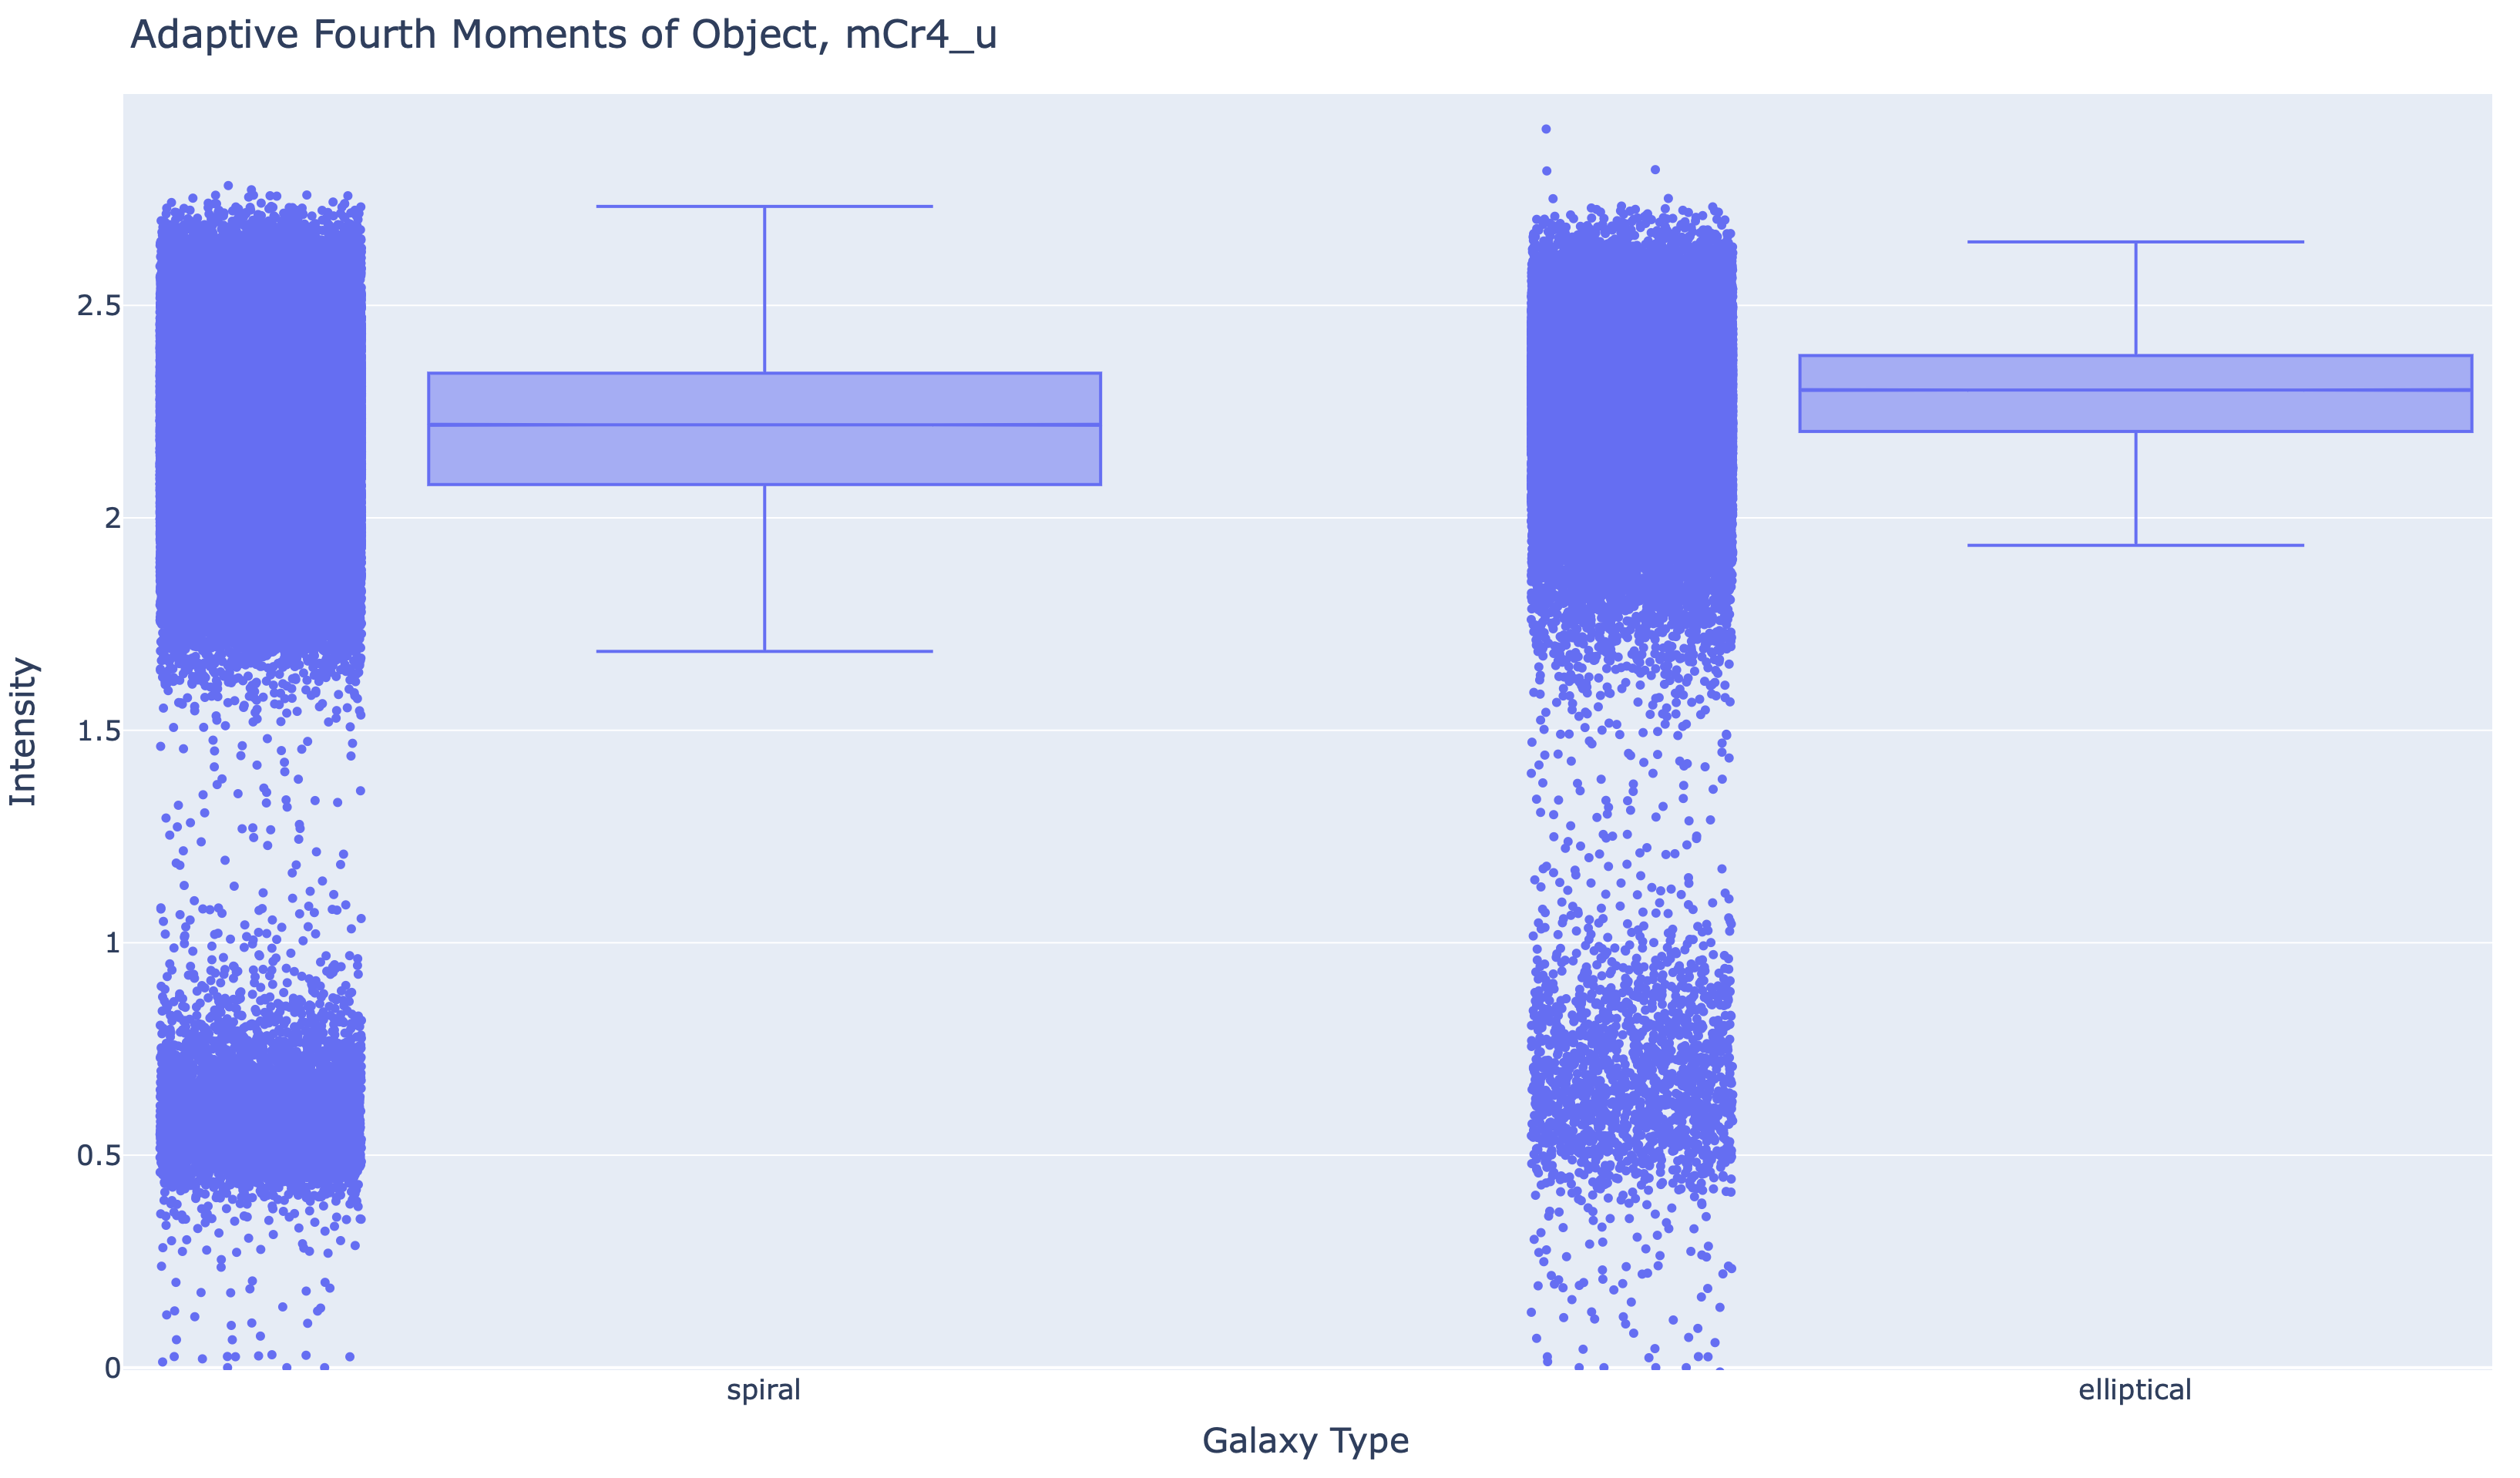
\includegraphics[scale=0.15]{mcr4_u_stat}
  \caption{Adaptive 4th Moments - mCr4u}
  \label{fig:mcr4_u_stat}
\end{figure}


\begin{figure}[htbp]
  \centering
  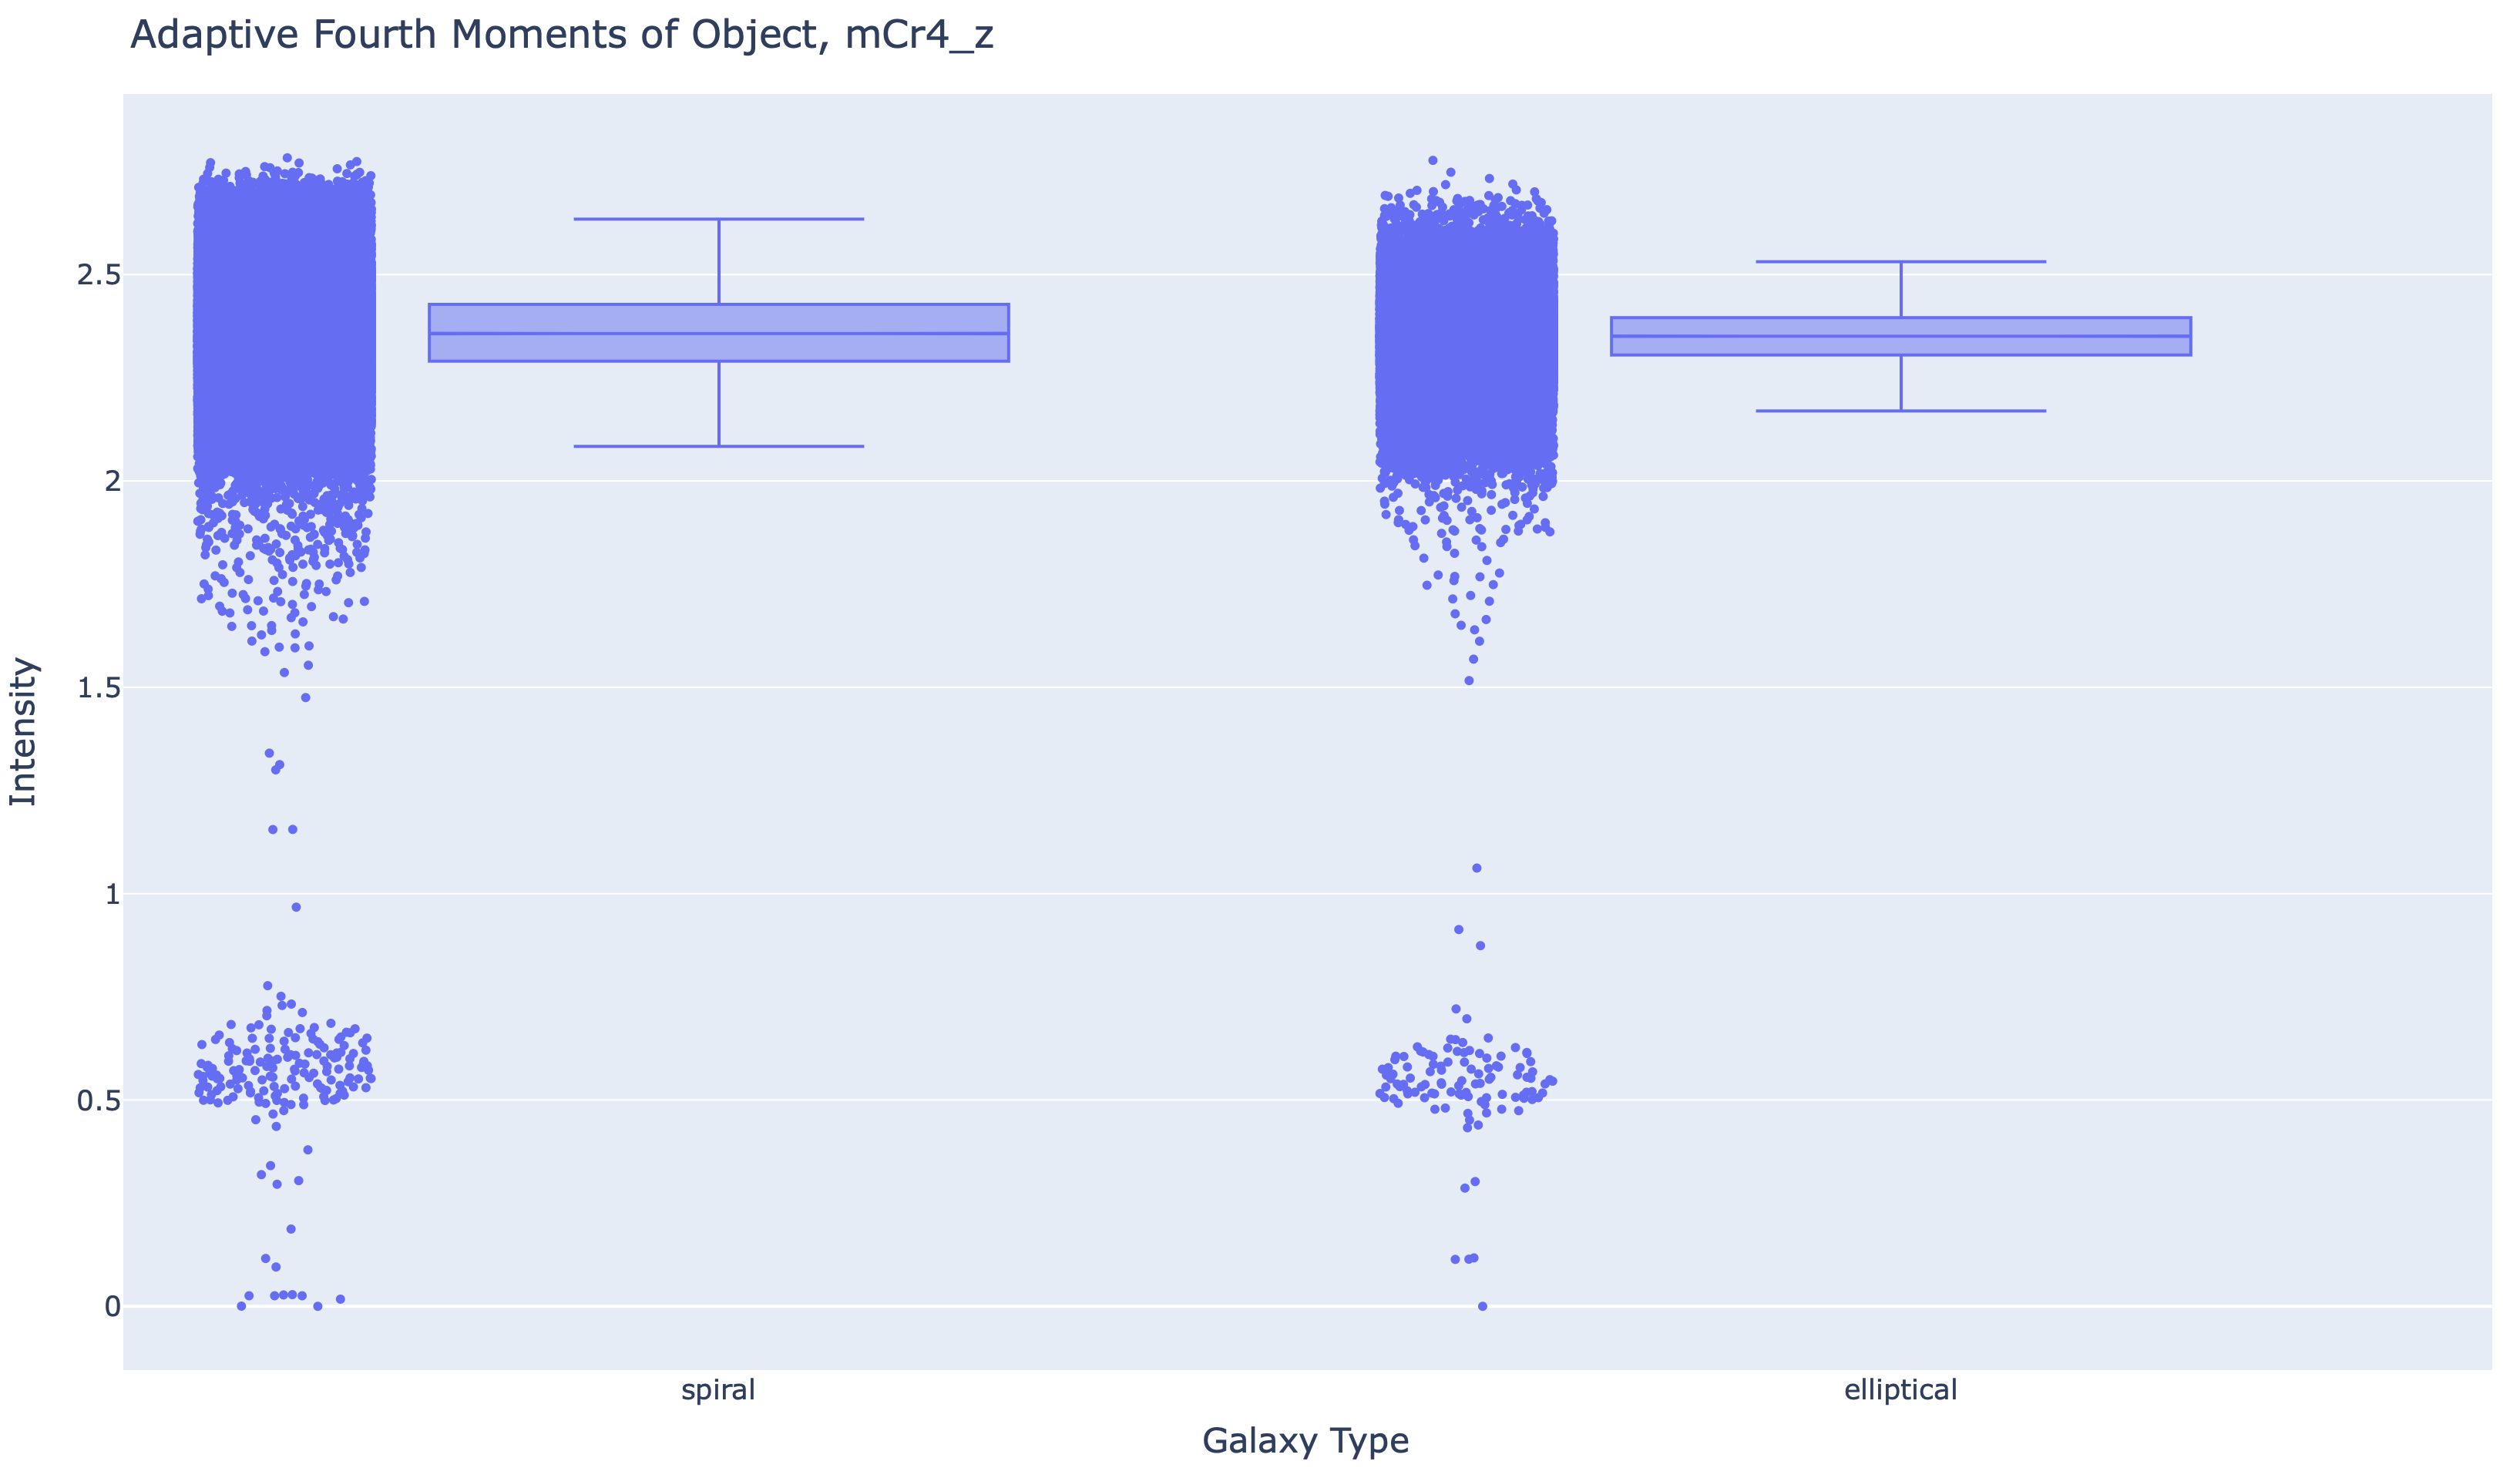
\includegraphics[scale=0.15]{mcr4_z_stat}
  \caption{Adaptive 4th Moments - mCr4u}
  \label{fig:mcr4_z_stat}
\end{figure}

\begin{figure}[htbp]
  \centering
  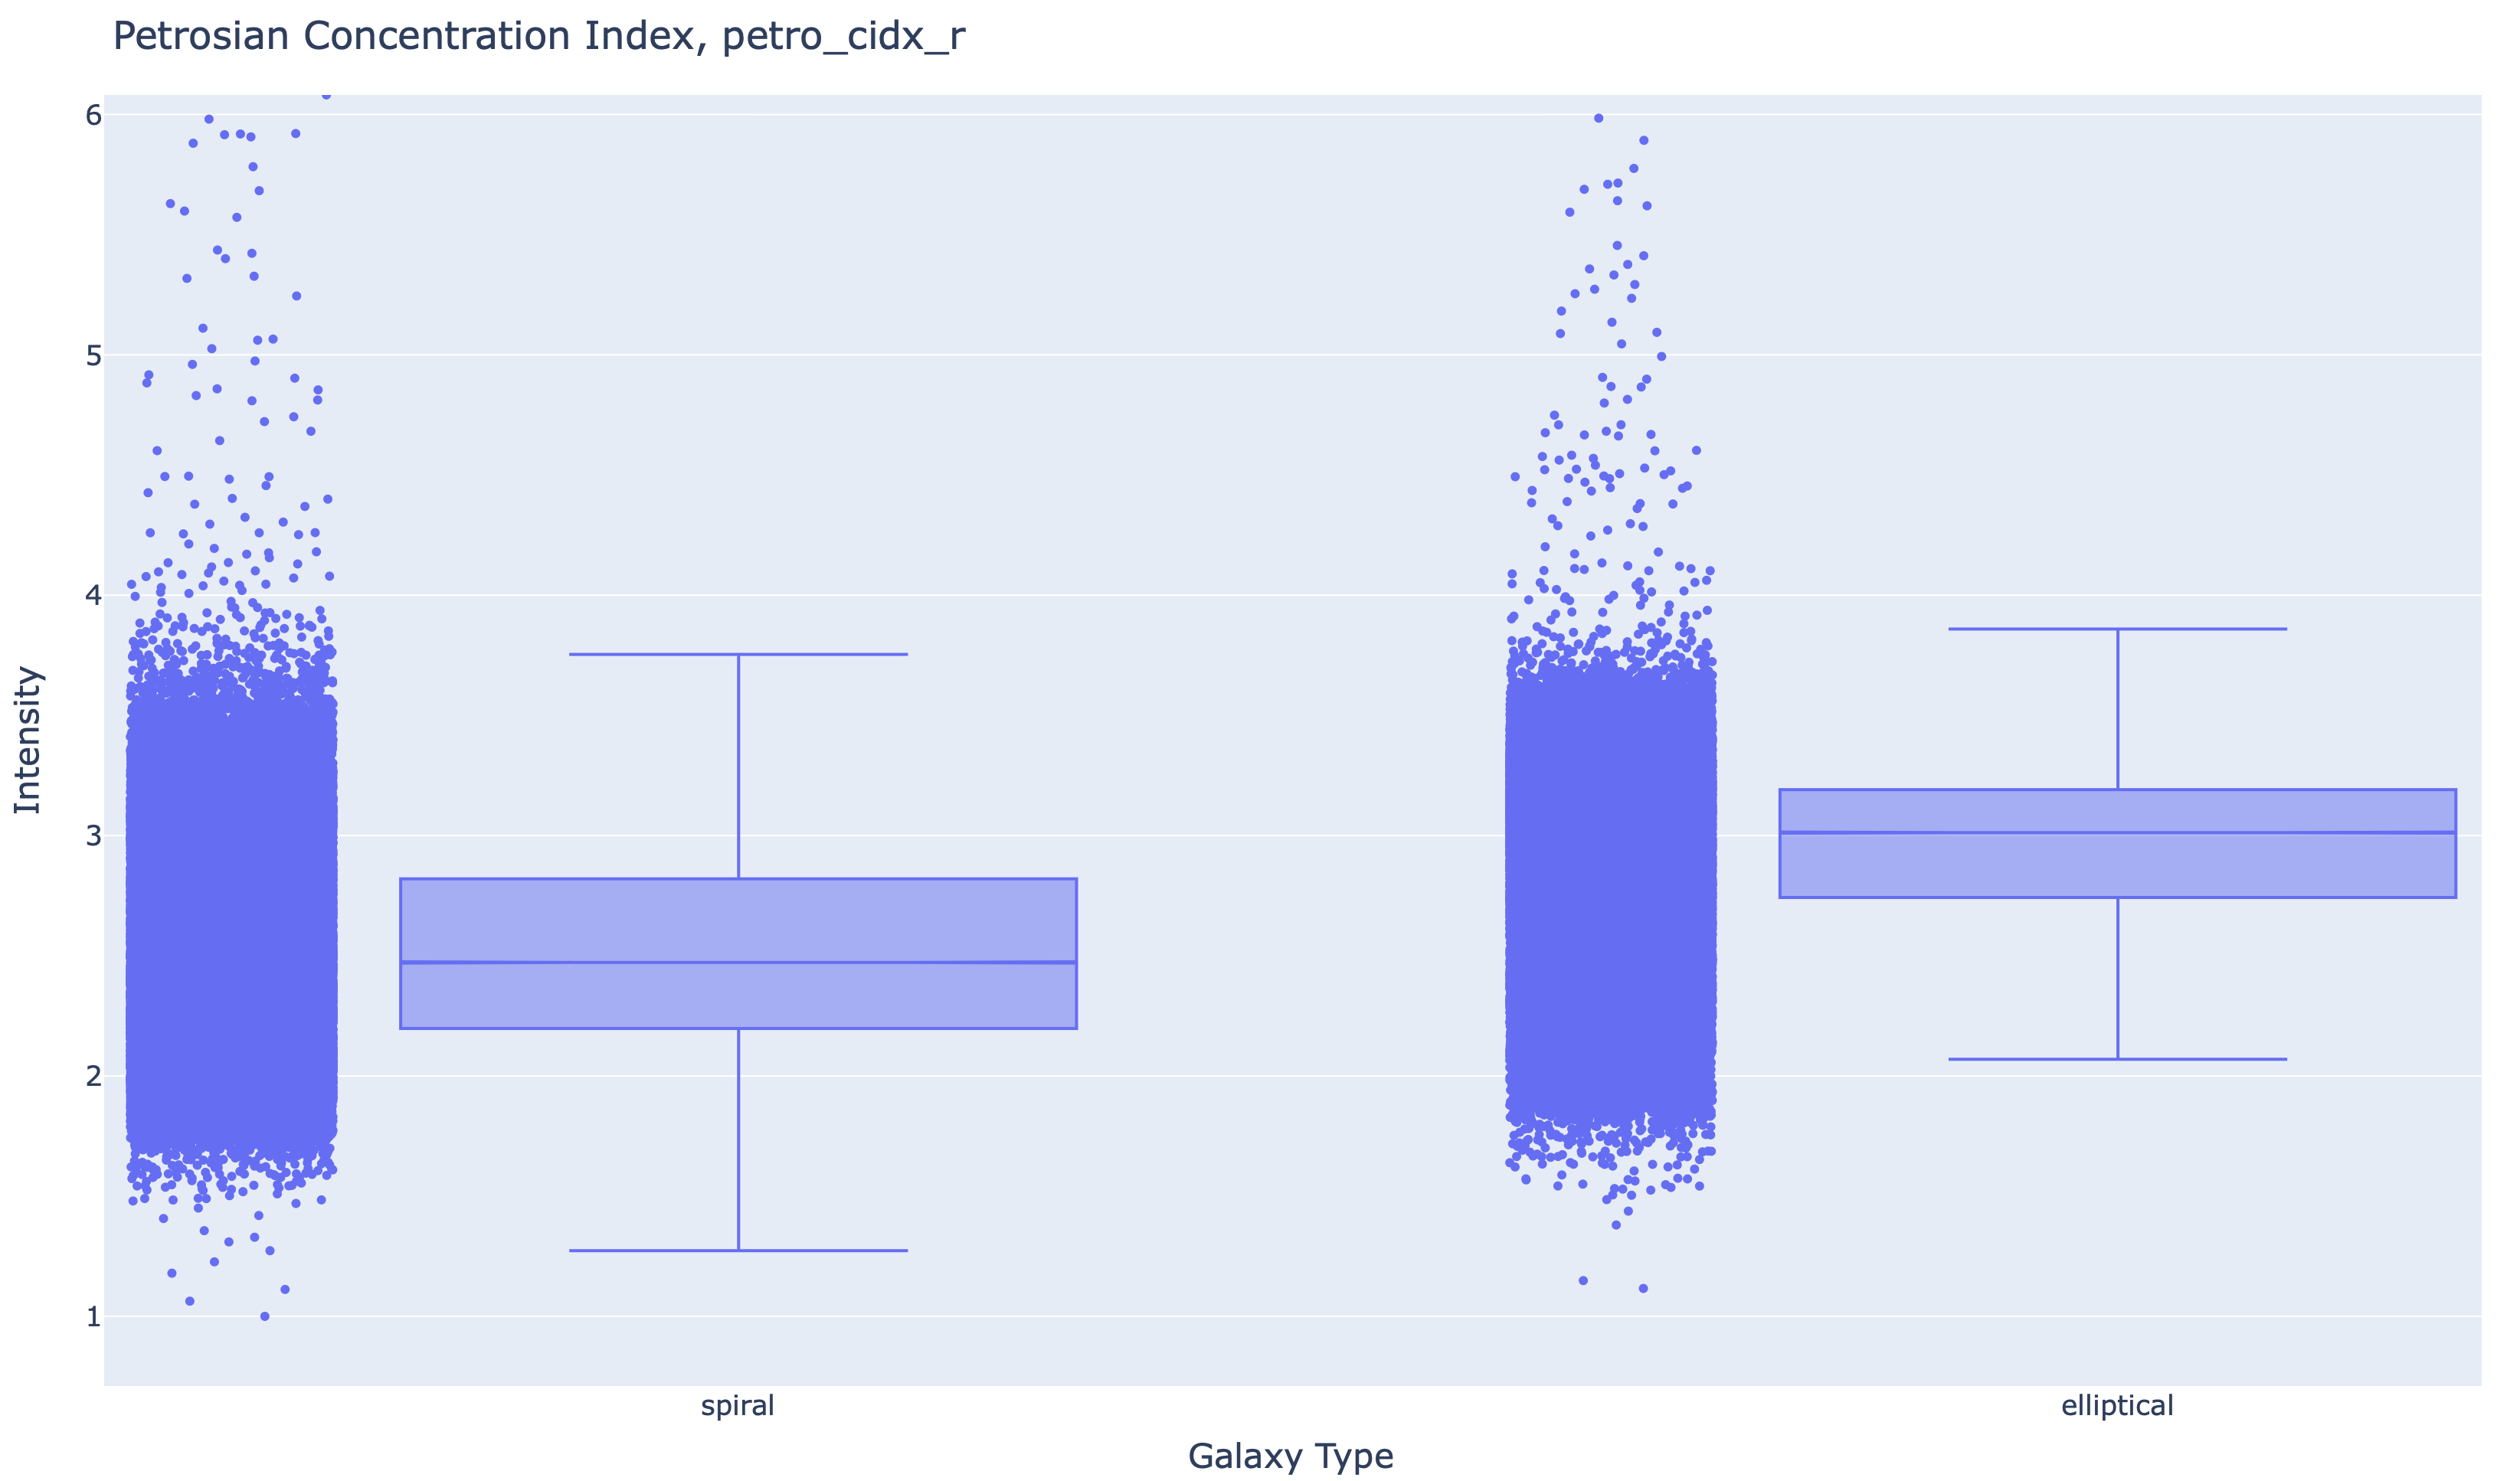
\includegraphics[scale=0.15]{petrosian_r}
  \caption{Petrosian Concentration Index, r}
  \label{fig:petrosian_r}
\end{figure}


\begin{figure}[htbp]
  \centering
  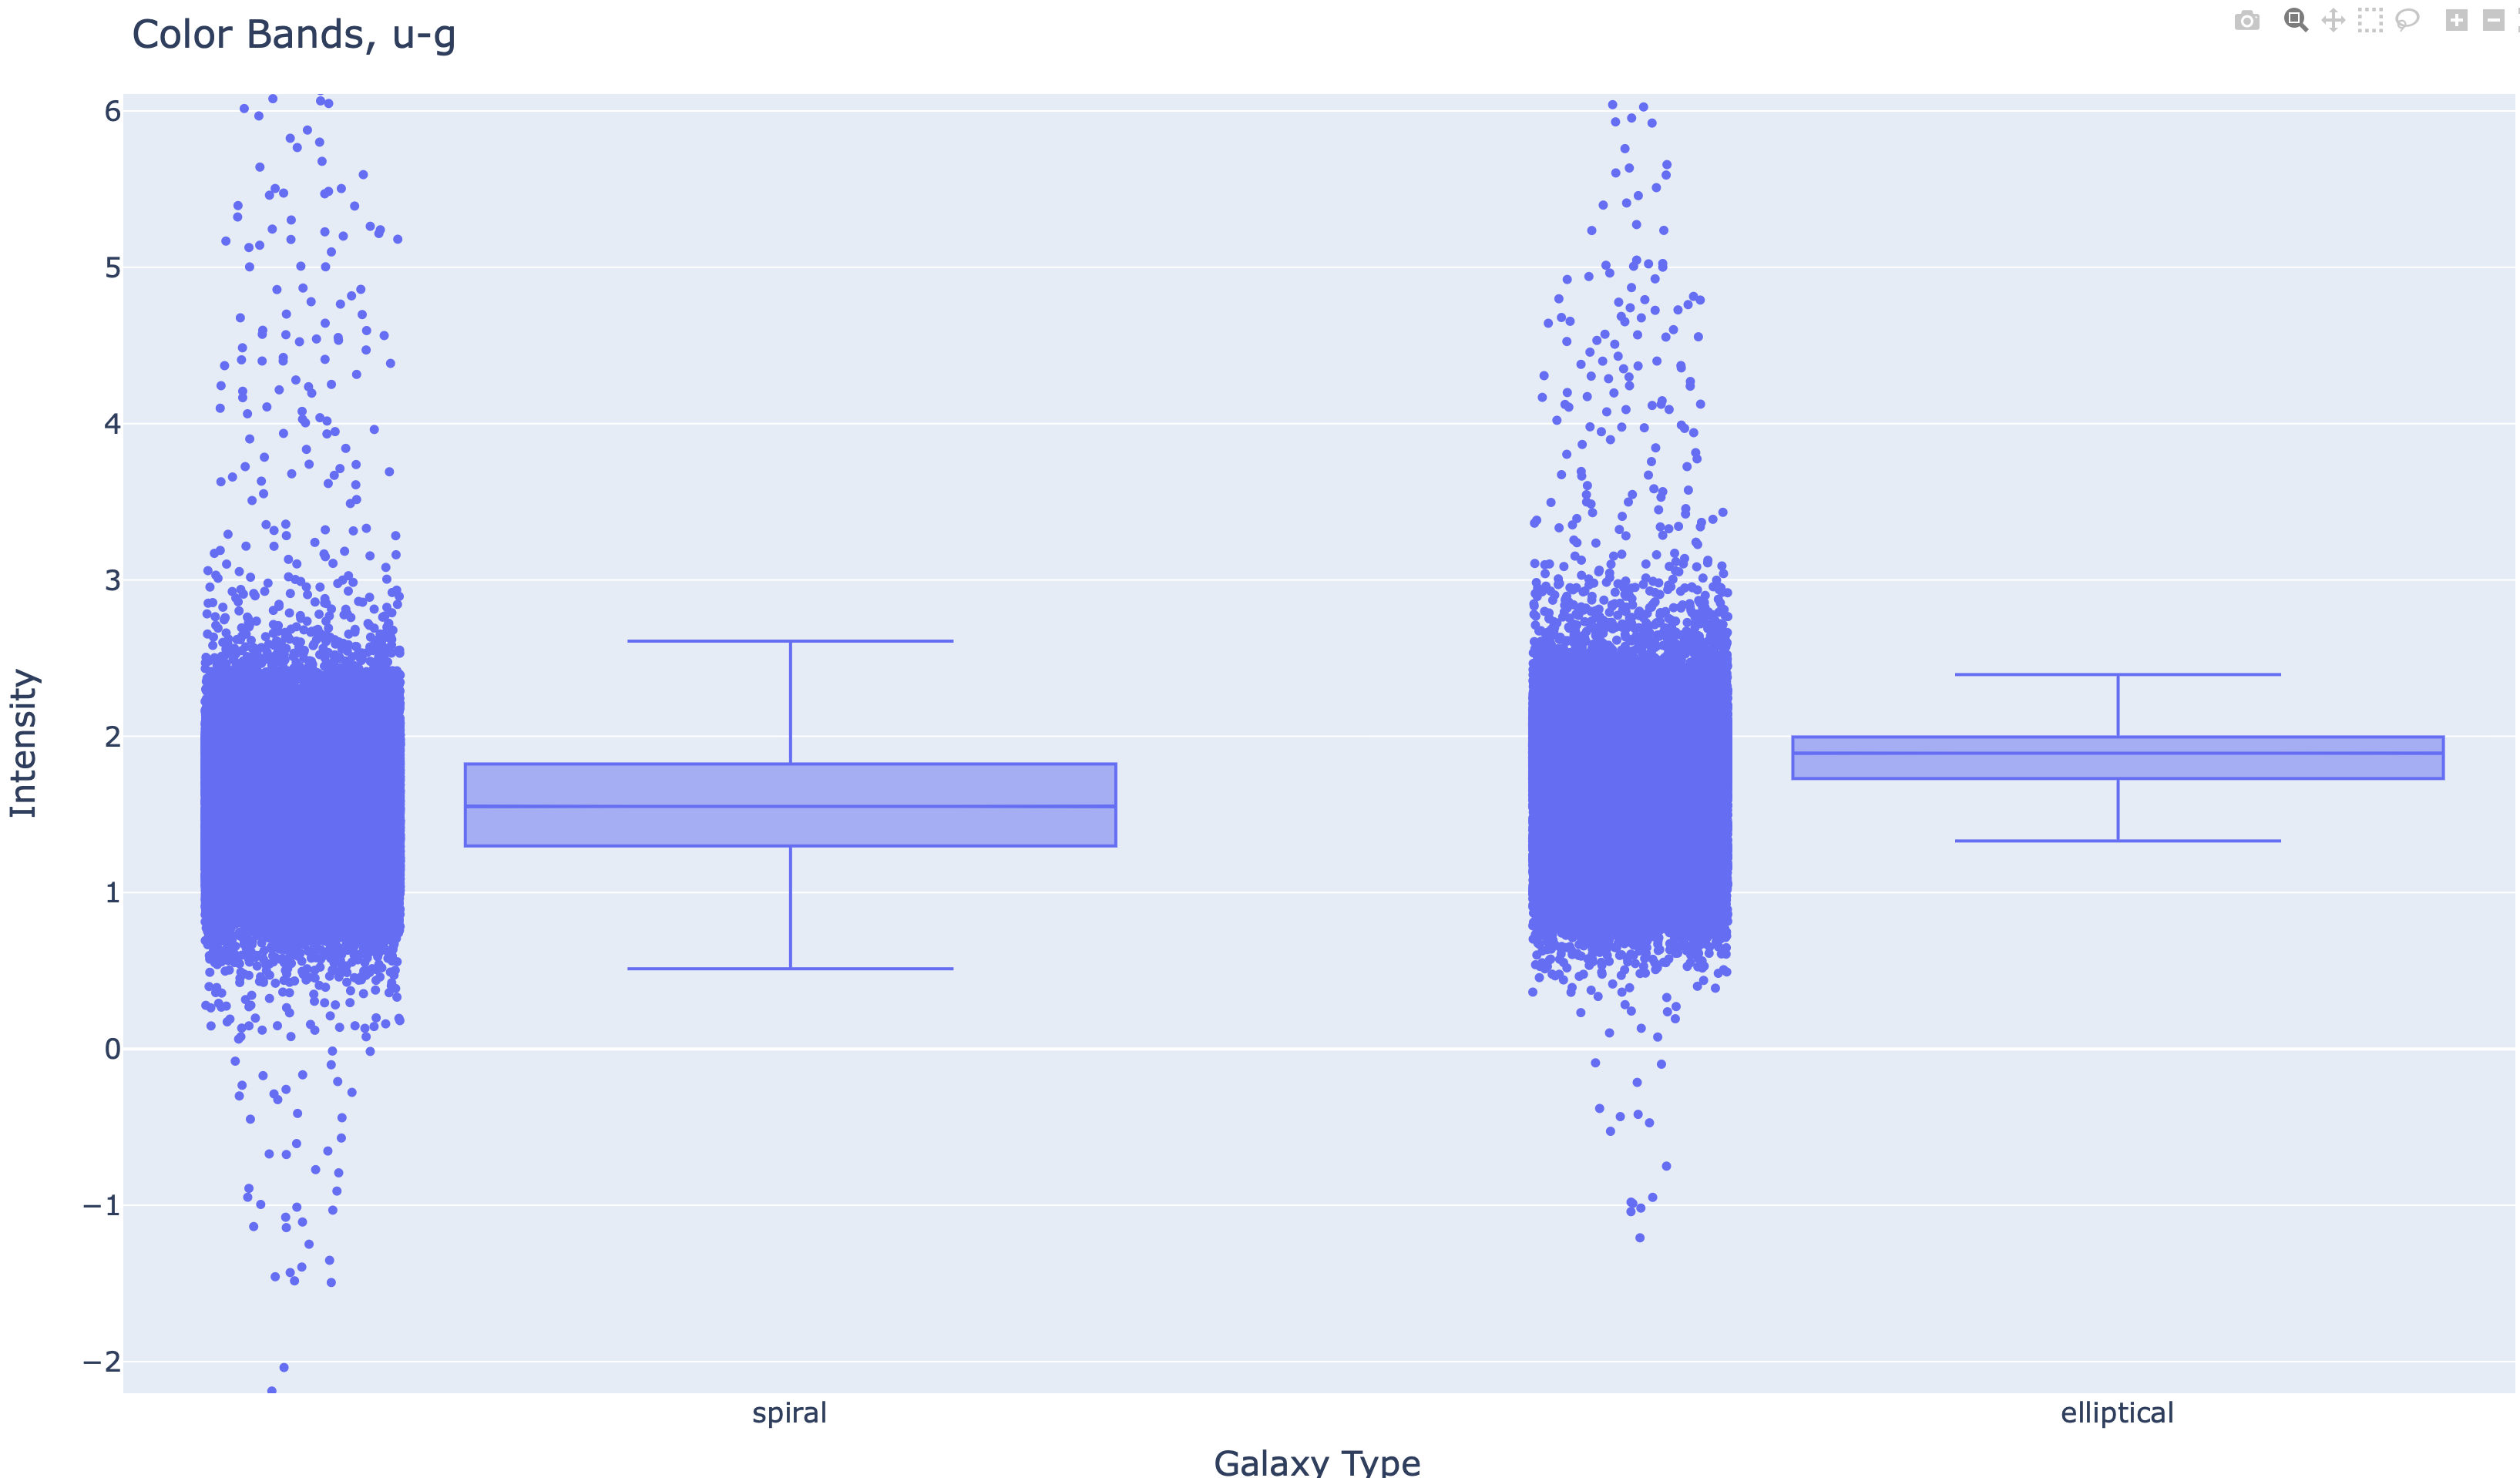
\includegraphics[scale=0.15]{ug_stat}
  \caption{Color Filter - u-g}
  \label{fig:ug_stat}
\end{figure}

\begin{figure}[htbp]
  \centering
  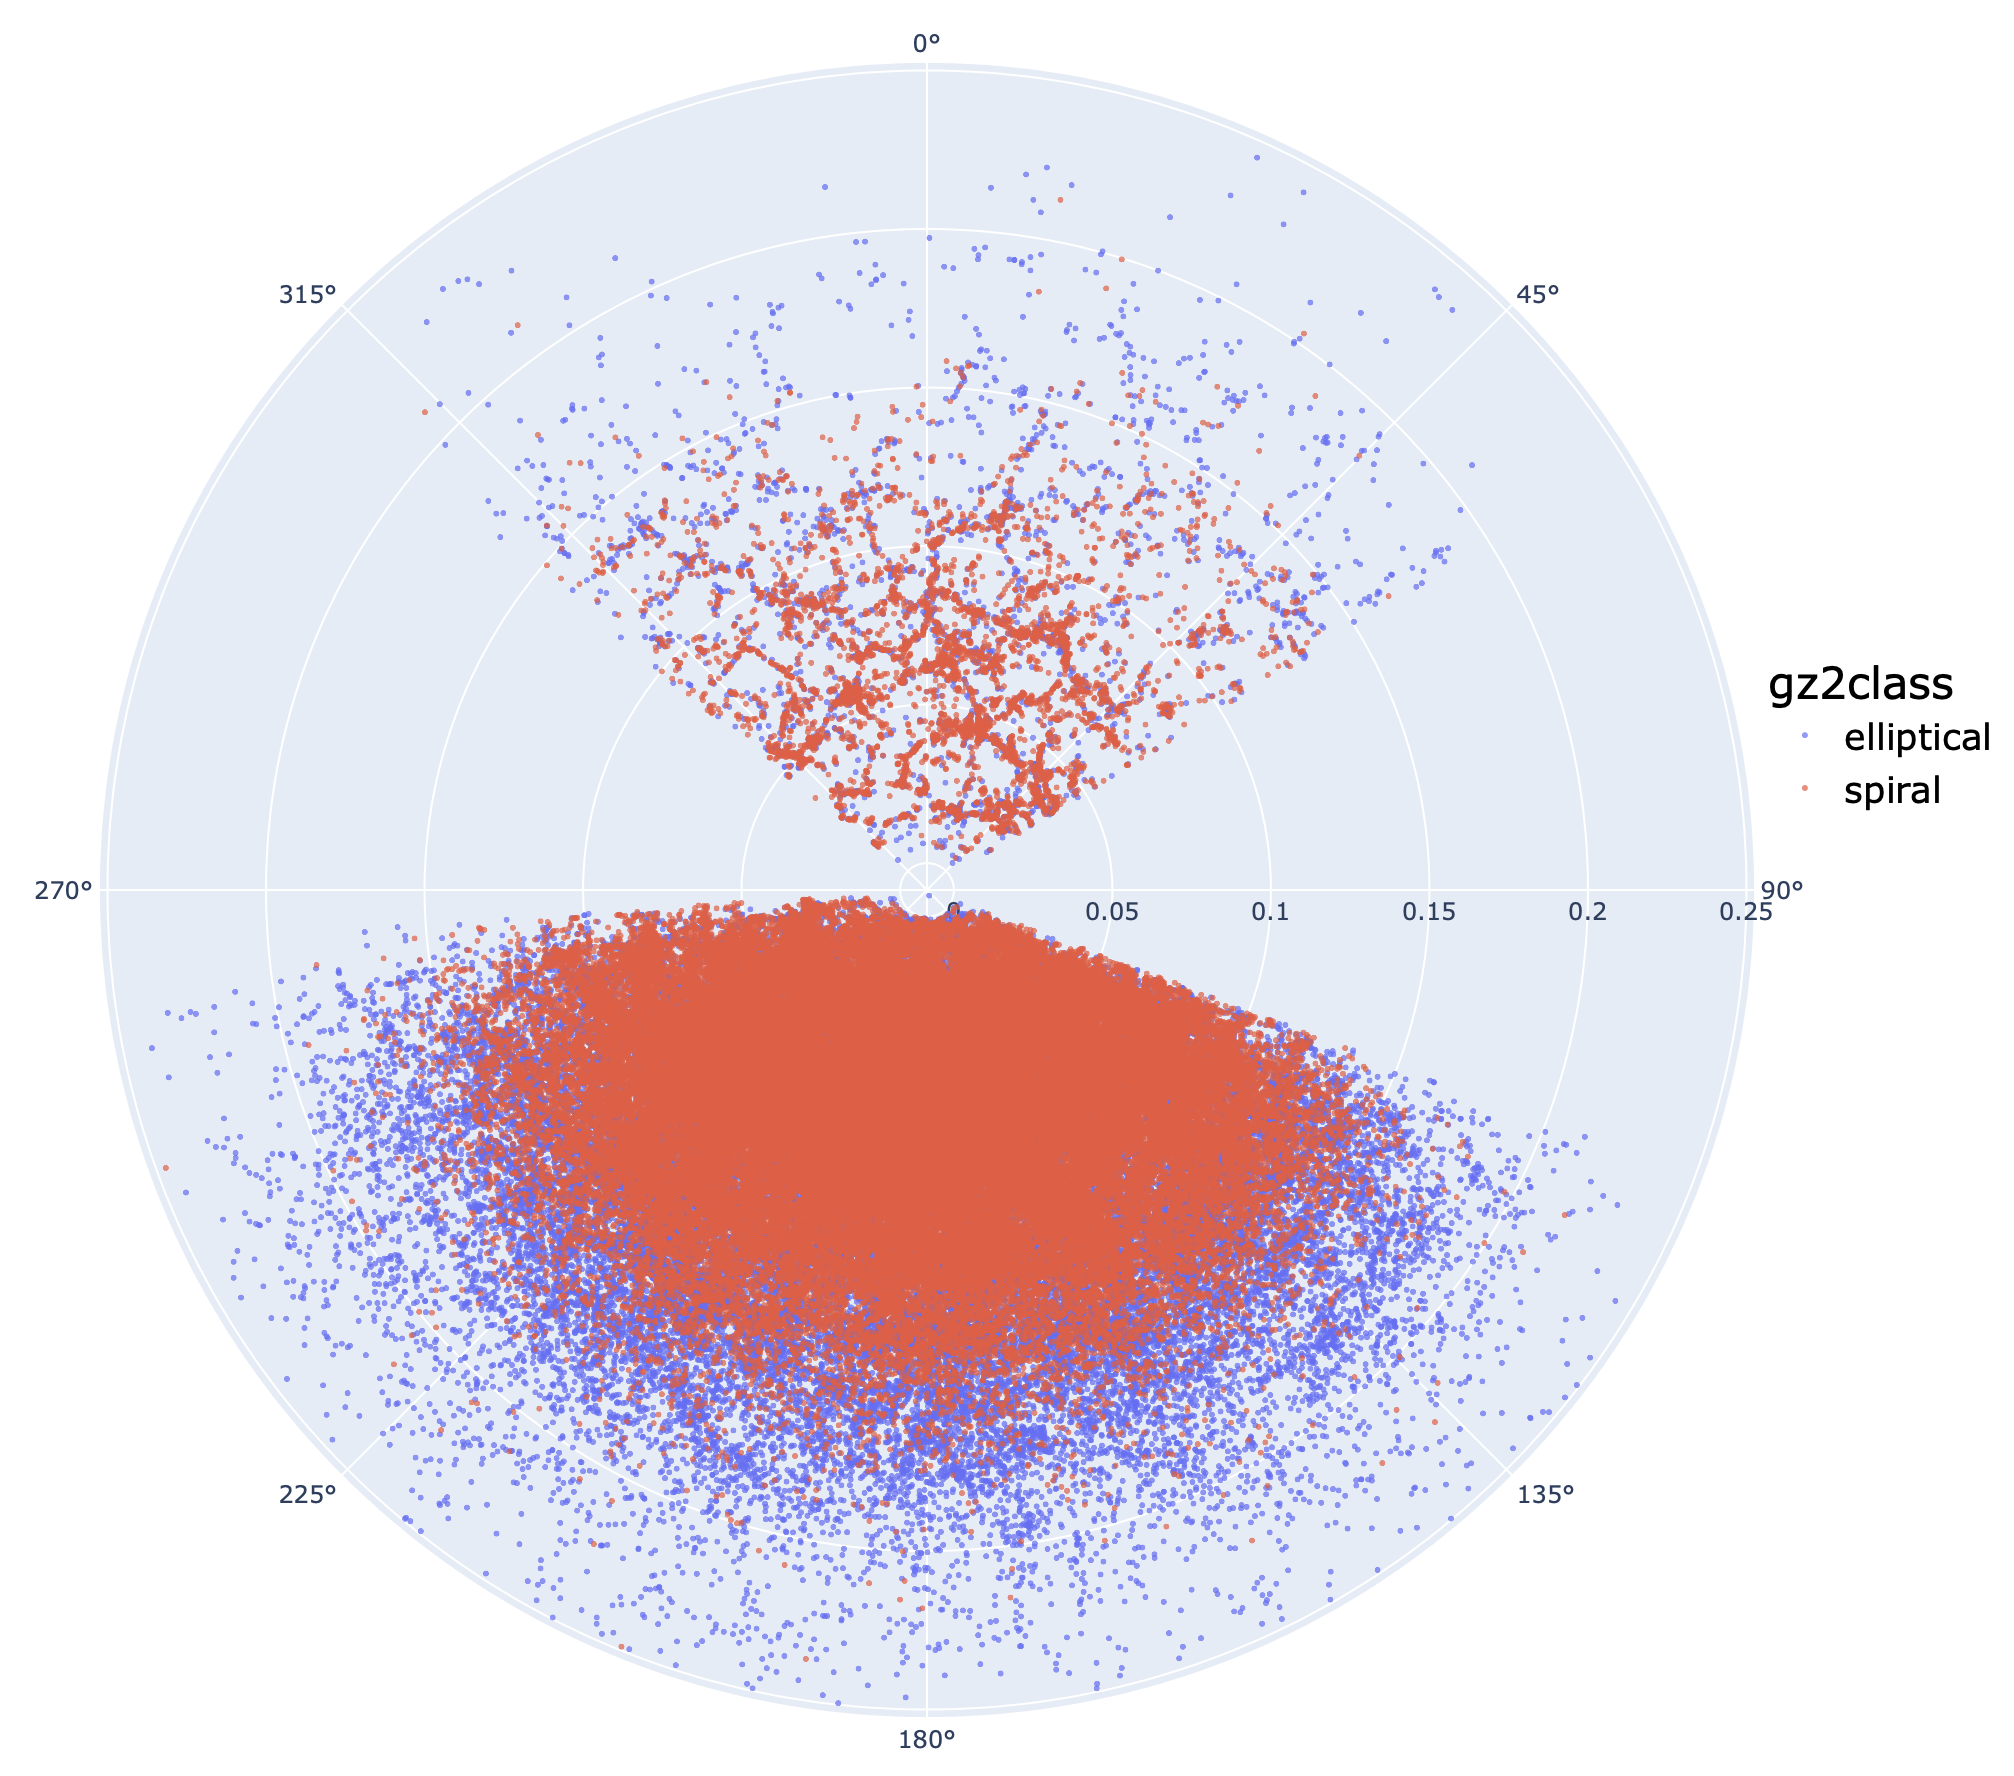
\includegraphics[scale=0.2]{redshift_polar}
  \caption{Redshift vs. Right Ascension}
  \label{fig:redshift_polar}
\end{figure}


\subsection{Machine Learning}

\begin{figure}[htbp]
  \centering
  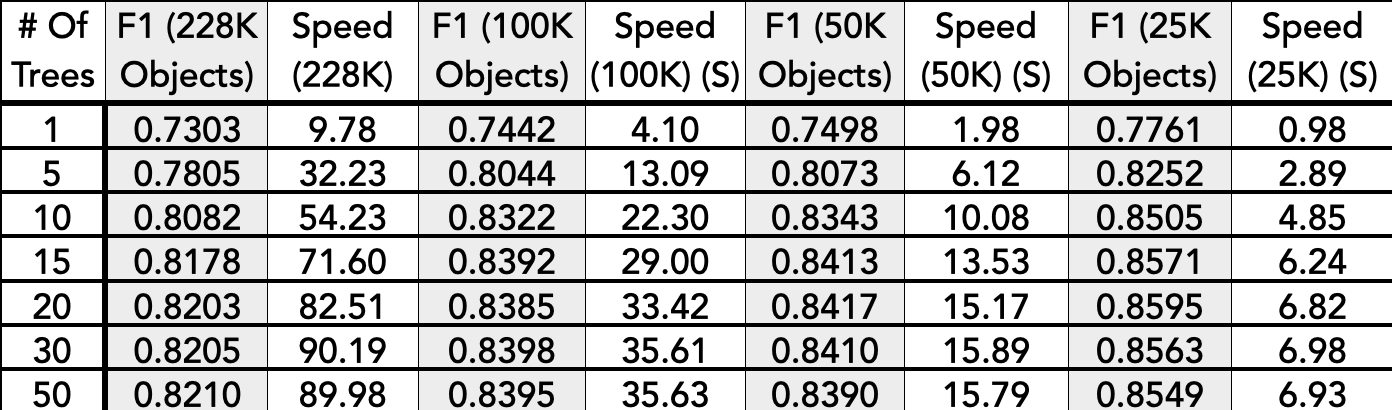
\includegraphics[scale=0.35]{randomforest}
  \caption{Random Forest Results}
  \label{fig:randomforest}
\end{figure}


\begin{figure}[htbp]
  \centering
  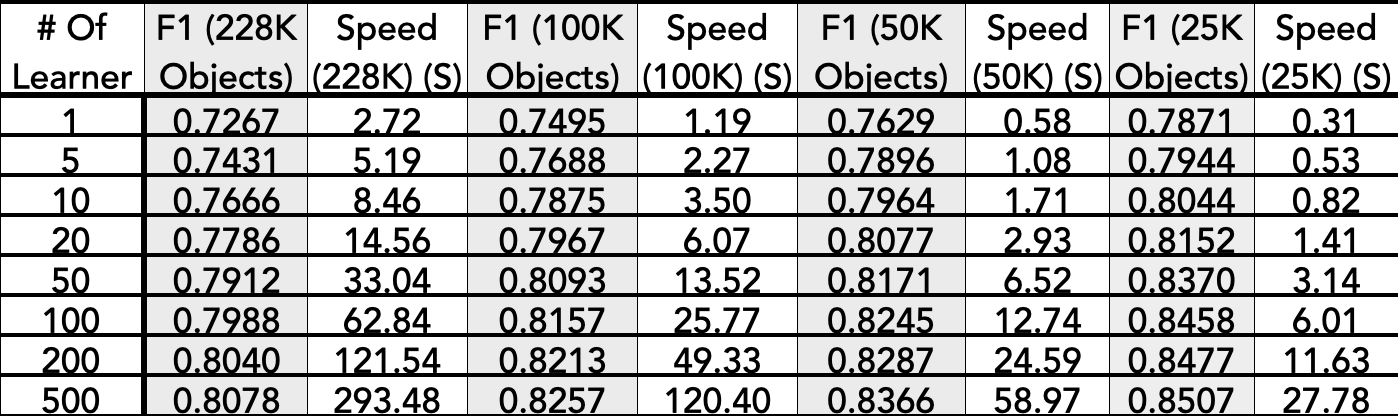
\includegraphics[scale=0.35]{adaboost}
  \caption{AdaBoost Results}
  \label{fig:adaboost}
\end{figure}

\begin{figure}[htbp]
  \centering
  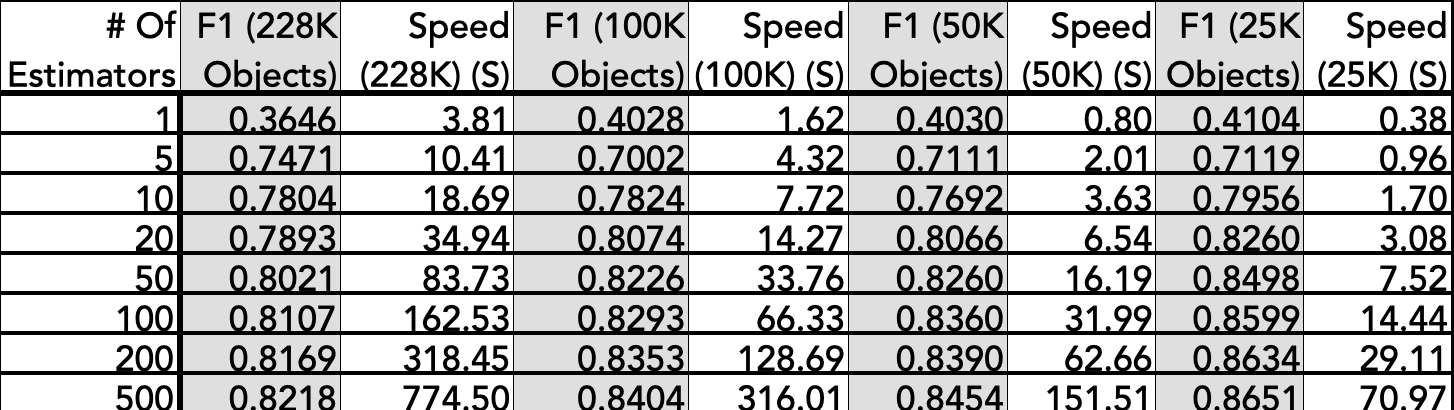
\includegraphics[scale=0.35]{stochasticboost}
  \caption{Stochastic Gradient Boost Results}
  \label{fig:stochasticboost}
\end{figure}

\begin{figure}[htbp]
  \centering
  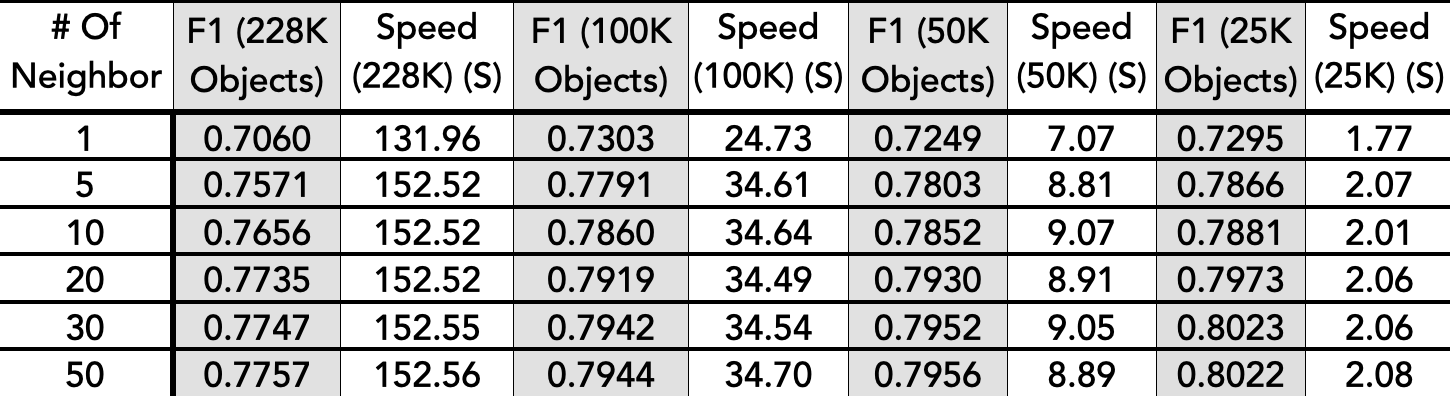
\includegraphics[scale=0.35]{knearestneighbors}
  \caption{K-Nearest Neighbors Results}
  \label{fig:knearestneighbors}
\end{figure}

\begin{figure}[htbp]
  \centering
  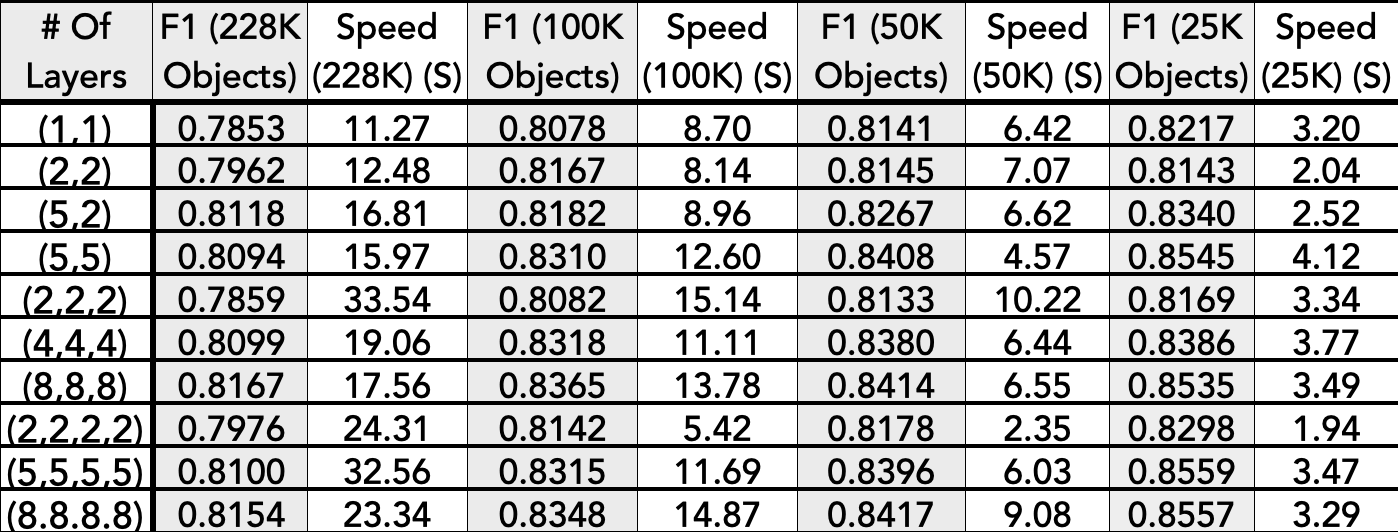
\includegraphics[scale=0.35]{mlpnn}
  \caption{Multi-Layer Perceptron NN Results}
  \label{fig:mlpnn}
\end{figure}




\section{Discussions}


\subsection{Results}


\subsection{Applications}


\section{Conclusion}


\section{Appendix}

Honor Code Pledge


\bibliographystyle{acm}
\bibliography{sigproc} 

\end{document}
